\documentclass[12pt, openany, twocolumn]{article}
\usepackage[utf8]{inputenc}
\usepackage[top = 1.5cm, left = 1.5cm, right =1.5cm, bottom = 1.5cm]{geometry}
\usepackage{graphicx}
\usepackage[pdfborder ={0 0 0}]{hyperref}

\title{In which way the use of virtual reality increases the efficiency of a learning process ?}
\author{ Aurélia Besse, Etienne Duverney, Jean-Guillaume Ponsard, Romain Junca }
\date{April 2019}

\begin{document}

\maketitle

\section{Context} 
\hspace{0.5cm} 
This document is presenting the articles and the context leading to the problematic for our research project about Virtual Reality for human rehabilitation and learning.
% Insert quote with the parallel between rehabilitation and learning
Past studies showed that learning and rehabilitation are linked thanks to muscular and memory training in both fields (medical and general). 
Indeed, learning systems based on immitation enhance motor learning in healthy and disabled individuals \cite{holdenUseVirtualEnvironments, bastianUnderstandingSensorimotorAdaptation2008b}.
Memory games have proved to be efficient in rehabilitating of brain functions lost in stroke accidents. From a past exprience, we can say patients improved their memory ability unexpectedly while enjoying playing the game.\\ 

As we do not have the required medical knowledge, we will demonstrate our statements with casual exercices.  
These exercises train the same parts of brain and muscles as some rehabilitation trainings.
Thus we can admit the benefits brought up in the medical field too.
\\

The Virtual Reality (VR) technology is an interactive computer-generated experience taking place in a simulated environment. 
Nowadays, the VR technology is composed of a head-mounted display and 3D audio headphones.
This technology allows a fully immersive experience for the user \cite{sveistrupMotorRehabilitationUsing2004}.
\\

Virtual Reality has been commercially available since the late 80's, with the first systems sold by VPL Research.
This technology has always evolved through time thanks to better computer technologies and better softwares.
This contributed to the "rebirth" of the VR in the late 90's \cite{burdeaVirtualRehabilitationBenefits2003} and later in the late 2010's.
\\


With the development of low-cost devices, this rehabilitation can be continued at home, easing the access to these tools, in addition to their ludic and thus motivating properties.
Indeed, motivation plays a major role during the learning process, as it helps to get quick and better results \cite{kangBenefitRetrievalPractice2014, christophelRelationshipsTeacherImmediacy1990, kinzieRequirementsBenefitsEffective1990b}.
Recent technological advances have led to considerable cost reductions for VR equipments, and several companies are selling headsets that consist of 2 lenses and a place to insert a smartphone for less than \$20 \cite{araneVirtualRealityPain2017}.
A relatively lowpriced virtual-reality-based training program would be a more effective and cheaper way to exercise than attending a class in sport center \cite{kimEffectsVRbasedWii2014}.
The democratization of the technology also allows the telerehabilitation \cite{burdeaVirtualRehabilitationBenefits2003}. This means a patient can be treated by professionals from all around the world. 
\\

Within Medicine, VR has been used in teaching anatomy, training in diagnostic procedures, in rehabilitation, teaching open and minimally-invasive surgery procedures.  \cite{burdeaVirtualRehabilitationBenefits2003}.
Virtual Reality system can provide multimodal stimuli, such as visual and auditory stimuli, and can also be used to evaluate the patient’s multimodal integration and to aid rehabilitation of cognitive abilities \cite{bioulacQuApportentOutils2018, morelAdvantagesLimitationsVirtual2015}. 
VR is similar enough to reality to provide an effective training environment for rehabilitation.
\\

In rehabilitation therapy, where repetitive feedback and motor learning are necessary, a virtual reality system can provide adequate motivation of such a mechanism \cite{kimEffectsVRbasedWii2014}.
In the medical field, VR has been used for the training of surgeons \cite{laverVirtualRealityStroke2017} or for the treatment of phobias \cite{morelAdvantagesLimitationsVirtual2015}. The secure environment allows to control the stimuli presented to the patient so he can face his fear gradually \cite{morelAdvantagesLimitationsVirtual2015}.
Also, recent reports have described the use of virtual reality (VR) as a method of distraction during procedures such as administering vaccines or drawing blood \cite{araneVirtualRealityPain2017}.
\\

In multiple articles we learn that the comparison between rehabilitation with or without VR proved that patients using this technology were more motivated and showed high levels of compliance during the process of rehabilitation \cite{sampaioDoesVirtualRealitybased2016, chenProgressSensorimotorRehabilitative2014}.
We can also notice that these patients showed better results and progress during these tests \cite{corbettaRehabilitationThatIncorporates2015, saposnikEffectivenessVirtualReality2010, chenProgressSensorimotorRehabilitative2014, saposnikgustavoVirtualRealityStroke2011}.
For example, these studies suggests a 5 times higher growth of chances of improvement in motor strength for patients who experienced a stroke after using a VR system \cite{saposnikgustavoVirtualRealityStroke2011}.
However, there is still work to do because, despite the number of studies about the benefits of VR in medical rehabilitation, and the number of patient who used it, and even the improvement observed, it is still not enough to prove that this method is 100\% better than the usual methods \cite{saposnikEffectivenessVirtualReality2010, saposnikgustavoVirtualRealityStroke2011, luque-morenoDecadeProgressUsing2015}.

\section{Experiment}

During our experiment, we want to demonstrate multiples improvement related to this technology:

\begin{itemize}
    \item The efficiency of VR excercices that require memory, movement precision and speed.
    \item The precision of the results implying an easiness of calculation of the different parameters (max level/reaction time/...).
\end{itemize}

    \subsection{Participants}
    % 10-20 personnes
    % tranche d'age : 15-30 ans & 45-60ans ?
    % sexe : homme et femme
    % pas d'handicape visuel ou moteur

    For the experience, we will ask around 15 persons to take the test. 
    Their age should be between 15 and 30 years old. 
    We take men and women indifferently because we are treating symptoms, not a illness, which could have different effects on different genders.
    These persons should have neither physical or mental handicap. 
    \\

    \subsection{Protocol}
    The idea is to evaluate the differences between a task done using a virtual reality system, and the same kind of task, but without the use of VR.
    A person is assisting the user during the test.
    \\

    For this, we used the same concept as a famous board game, the "Simon".
    We used a physical version of the board game, and the same version in a virtual reality environment.
    \\

    This study will be splited between three groups. One testing only the physical version, another testing only the VR version and the last group testing both.
    For the last group, there will be a time between each test in order to avoid study bias. We use this process in order to have the clearest results as possible (Results for the physical game only/Results for the VR game only/Results for both versions), and to really see the impact of the two versions. 
    \\

    In the physical version, as can you see in the figure 1 above, we have four differents colors, which light one after another, producing a different sound for each color.
    \\
    
    \begin{figure}
    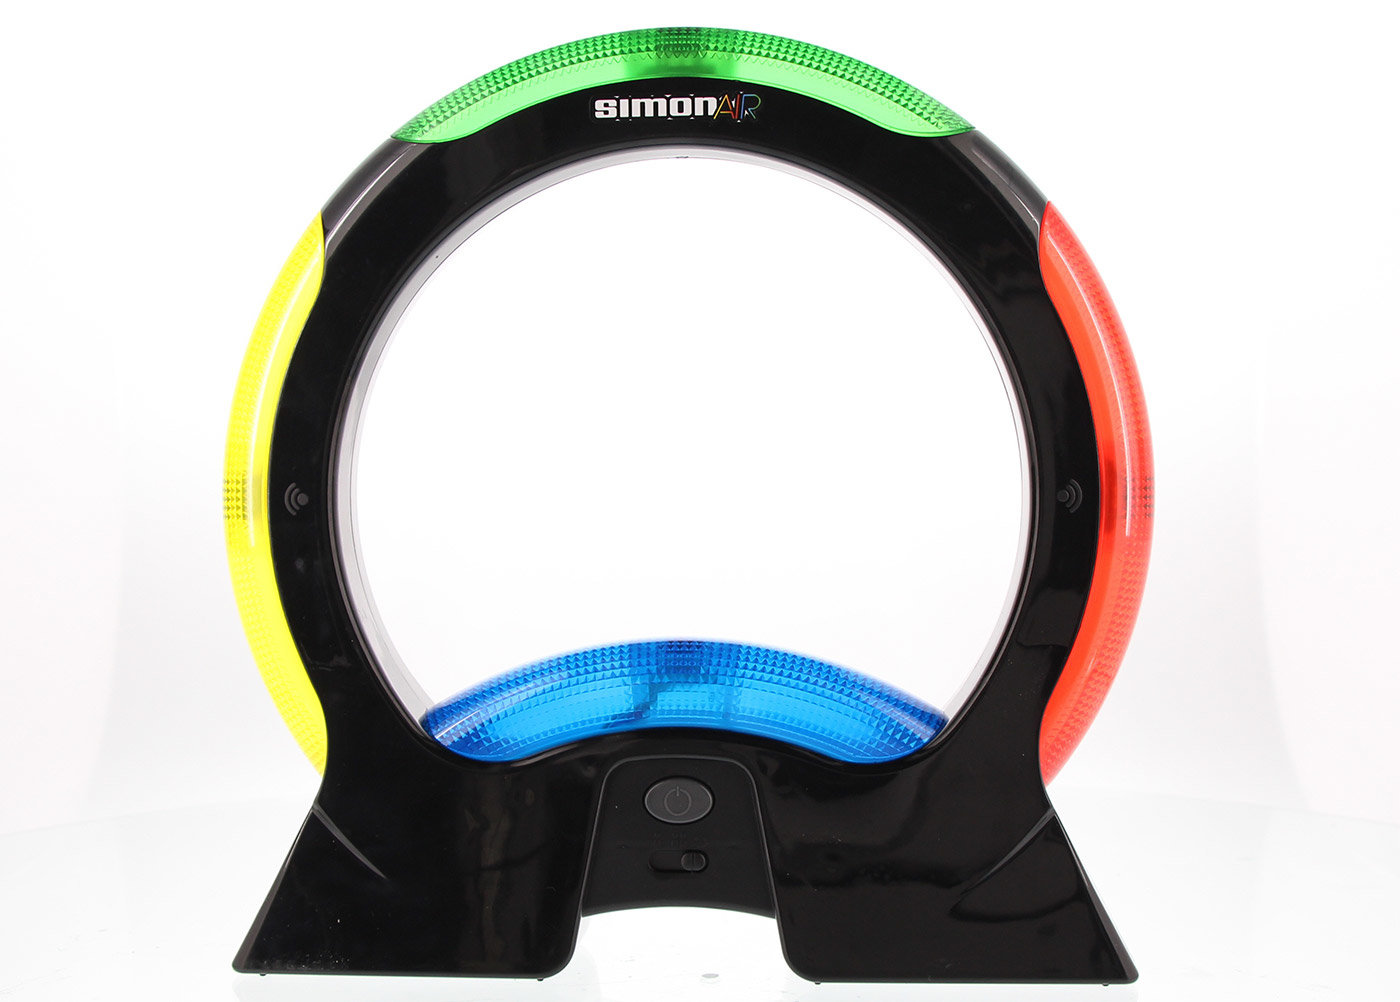
\includegraphics[scale=0.185]{simon.jpg}
    \caption{The Simon game}
    \end{figure}

    The goal for the user is to memorize the order in which the buttons lighted, and reproduce it by moving his hand in front of each color (a sensor will detect the hand of the user).
    After succeeding it, the same sequence will restart, but there will be more buttons's lightning than before.
    The longer the sequence will grow, the harder the game will be.
    If the user fails to reproduce the sequence exactly, the game is over.
    \\

    We developed the same game but in a virtual reality environment, in which the concept is the same and the player uses the controller of the VR-system to select a color.
    \\

    For the first group, we used the physical version of the game.
    While a person is playing, a second person (the operator) will write down the different parameters we need for the data analysis (see \ref{data}).
    For the second group, we used the same version of the board game but in the VR environment.
    We don't need an operator here, the application will automatically register the needed data.
    Finally, for the third group, we first used the physical version. Then we waited one week before making them play the VR game. Indeed, if they directly try the VR version right after this, it could change their way of playing the game in the VR environment (they would be more efficient).
    At the end, we compare the data of all of the three groups.

    \subsection{Data Analysis\label{data}}
    %All these statistics will be measured by the VR captors and environment.
    
    %- Speed : How long does it take  for the user to reproduce the sequence (comparing to the actual duration of the original sequence) ?
    %- Efficiency: How long is the sequence remembered by the patient ? Difference between the first session and the Nth session.
    %- Accessibility :  How easy it is to install, and play the game ? To record the data ?

    
    %speed    
    We will measure the speed of action because it is one of the main statistics we want to improve when rehabilitating. 
    We will measure here the physical speed, which can be defined by the quickness of movement of the hand toward the zone to hover.
    If the training is successful, we should see an improvement in the patient's speed of execution of the different exercises.
    \\

    %efficiency
    We will also measure the mental speed, or efficiency of the training. 
    If the training is successful, we should see an improvement in the amount of color the patient is able to memorize before finishing the game.
    \\

    %accessibility
    The training, supposed to be done at home by anyone, should be easy, from the setup of the environment to the actual beggining of the game. 
    We can measure here the time spent on the different interface pannels and how much time the user spends to setup the machine, with the help of our instructions.

    \subsection{Tools}
        \title{\textbf{The Simon game}} \\
    The Simon game is a memory board game in which the player has to reproduce the order of lights displayed by the game by, in our version, putting his hand over the required color. \\

        \noindent \title{\textbf{Virtual Reality Headset/Controllers (HTC Vive/Oculus Rift)}} \\
    With these systems, we are able to create a simulated environment we can control and in which the user can interact. \\
    
        \noindent \title{\textbf{Unity3D}} \\
    A real-time engine developed by Unity Technologies we used to develop (using the C\# language) the 3D environment, allowing user interactions and data analysis. \\

        \noindent \title{\textbf{Blender}} \\
    A free open-source 3D computer graphics software toolset we used to create 3D model. For example here, we reacreated the shape of the Simon board game. \\   
        
        \noindent \title{\textbf{Timer}} \\
    Used by the operator to evaluate the time data of the current player. \\

        \noindent \title{\textbf{Paper/Pen}} \\
    Used by the operator to write down the observed data of the current player. \\
    
        \noindent \title{\textbf{Statistics Analysis}} \\
    Used to compile and compare our data.

\bibliographystyle{plain}
\bibliography{database}
\end{document}
